\documentclass{article}

\usepackage{times}
\usepackage{uist}
\usepackage[config, font=small, labelfont={sf,bf}, textfont=sf]{caption,subfig}
%\usepackage{setspace}
%\doublespace
%\usepackage[config, font=small, labelfont={sf,bf}, textfont=sf]{caption}
\usepackage{subfig}
\usepackage{graphicx}
\usepackage{float}

\begin{document}

% --- Copyright notice ---
%\conferenceinfo{UIST'11}{October 16-19, 2011, Santa Barbara, CA, USA}
%\CopyrightYear{2011}
%\crdata{978-1-4503-0716-1/11/10}

% Uncomment the following line to hide the copyright notice
\toappear{}
% ------------------------

\bibliographystyle{ieeetr}

\title{Sketch It, Make It: Freehand Drawing\\
for Precise Rapid Fabrication}

\author{
\parbox[t]{9cm}{\centering
	     {\em Author One}\\
	     Institution Name\\
             City, ST, USA\\
	     user@institution.net}
\parbox[t]{9cm}{\centering
	     {\em Author Two}\\
	     Institution Name\\
             City, ST, USA\\
	     user@institution.net}
}

\maketitle

\abstract We present Sketch It, Make It (SIMI), a design tool for
precisely creating models for laser cutting. SIMI provides a suite of
pen-based interaction techniques that let the designer fluidly
transition from rough ideas to precise output in a single tool. These
techniques include creating linework or stencils to cut, and gestures
that edit the model or apply geometric constraints. We present a
system evaluation, including a study involving 60 undergraduate
architecture students. The evaluation suggests that sketch-based
interaction can be used beyond the early phases of design, allowing
people to create complex objects that meet precise specifications.

\classification{I.3.5 [Computational Geometry and Object Modeling]: Modeling packages}

% TODO: change this
\terms{Design, Human Factors}

\keywords{sketching, rapid fabrication, design tools, constraints}

\tolerance=400 % prevent words from sticking out in the margin

%% \begin{figure}[tb]
%% \vspace{1.9in}
%% \caption{A figure caption.  It is set in 9 point Helvetica type, with a
%% 0.5 cm wider margin on both left and right sides.} 
%% \label{fig-example}
%% \end{figure}

\section{INTRODUCTION}

\begin{figure}[h]
\centering 
\subfloat[] {
  \label{fig:cintiq} 
  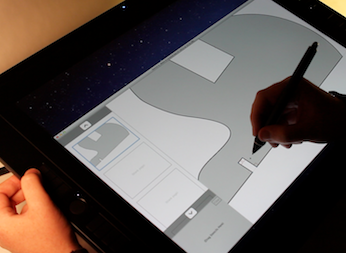
\includegraphics[width=0.6\linewidth]{img/simi-with-cintiq.png} % 0.65
}
\\
\subfloat[] {
   \label{fig:lg-pencil-holder}
   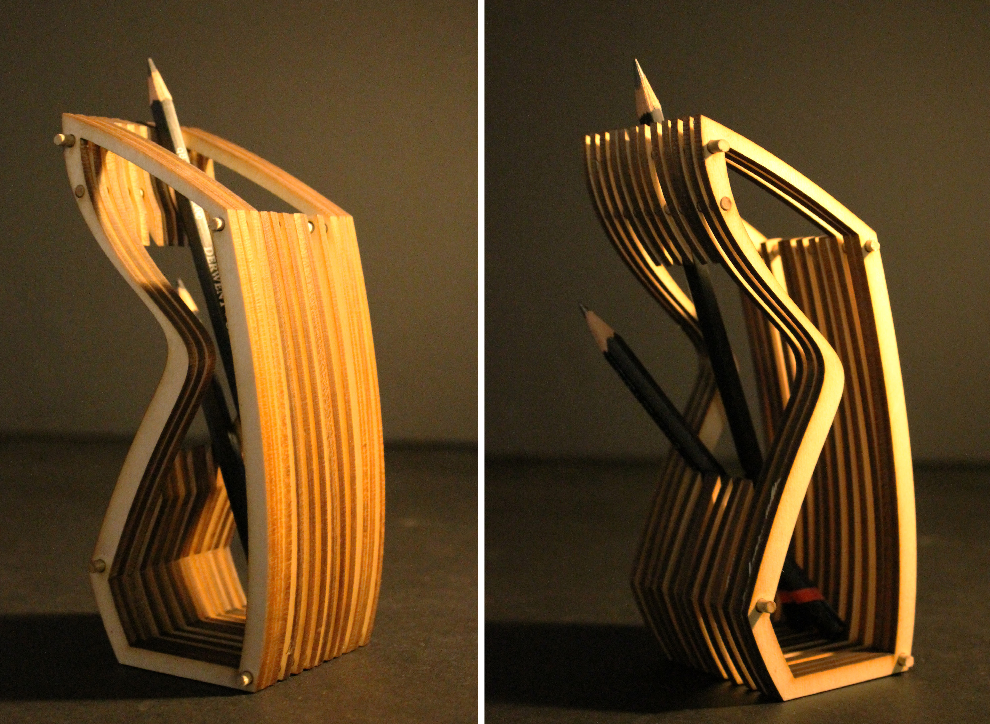
\includegraphics[width=0.6\linewidth]{img/lg-pencil-holder.png} % 0.9
}
\caption{Sketch It, Make It lets users design laser cut items with
  sketch-based interaction. \subref{fig:cintiq}: using SIMI with a
  Wacom Cintiq. \subref{fig:lg-pencil-holder}: laser-cut pencil
  holder designed by an undergraduate student using SIMI.}
\label{fig:simi-intro}
\end{figure}

A growing community of self-described \textit{Makers} design and build
many kinds of physical things~\cite{gershenfeld-fab}. Some are
electronic devices, while others are made entirely from traditional
materials. These ``new makers'' employ rapid fabrication machines such
as 3D printers, laser cutters, and other CNC machinery.

Laser cutters are among the more common and affordable fabrication
machines. Think of a laser cutter as a very fast, strong, and precise
automated razor, cutting flat material (paper, wood, plastic, metal,
etc.). Many things can be made with only a laser cutter, some fastened
with screws or glue. Figures~\ref{fig:simi-intro} and~\ref{fig:table}
show examples of laser cut objects.

Today, designers can choose from among several modeling tools for
laser cutter projects. The most common is Adobe Illustrator, a
general-purpose, full-featured vector graphics editor. New users find
its interface familiar (at least superficially) because it resembles
other applications they have used previously. Despite this sense of
familiarity, participants in our formative study (presented later) had
a hard time using Illustrator quickly and effectively. Avocational
designers need appropriate modeling tools~\cite{lipson-homefactory}.

We present ``Sketch It, Make It'' (SIMI), a modeling tool for laser
cutter design based on recognizing short sequences of input sketched
with a stylus. Using only freehand drawn input, SIMI enables a
designer to iteratively and incrementally create precise laser cut
models.

Research on sketch-based modeling tools~\cite{johnson-sketch-review}
typically views sketching as an activity done mostly in the early
phases of design. Tools based on this assumption are justifiably
oriented towards capturing imprecise input. Only a few sketch-based
systems support designers in later
stages~\cite{mori-plushie,saul-sketch-chair,naya-parsketch}.


% TODO: Mark asked for citations for the above statement about
% sketch-based systems that support late-phase design. I could offer
% ParSketch, Lineogrammer, Furniture Factory, SketchChair, and maybe
% dig up whatever is going on with Igarashi/Lipson/Stahovich labs. But
% as far as I know, this is not a very strong statement, as nobody
% that I know of really has a system that supports both fabrication
% *AND* human-in-the-loop precision.

We are inspired by the potential of freehand drawing as a basis for
precision modeling for several reasons. Sketching is quick and can be
easily learned. It is simple and modeless: unlike structured editing
software, a designer need not set a pencil's mode to line, circle, or
anything else. Yet (as we shall show), sketched input can provide
enough information to translate into a precise digital model.

\subsection{Motivating Example}

\begin{figure}[t]
\centering 
\subfloat[] {
  \label{fig:example-1} 
  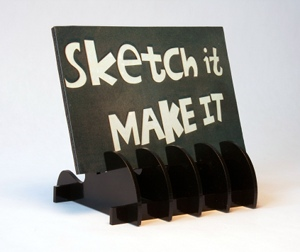
\includegraphics[width=0.45\linewidth]{img/simi-stand-withpic.jpg} 
}
\subfloat[] {
    \label{fig:example-2}
    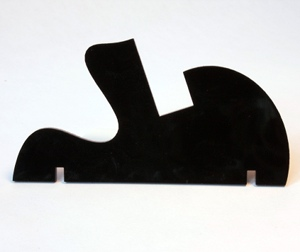
\includegraphics[width=0.45\linewidth]{img/simi-stand-part.jpg}
}
\caption{A picture stand \subref{fig:example-1} drawn and fabricated
  using SIMI. A single copy of the primary part is shown in
  \subref{fig:example-2}. }
\label{fig:simi-example}
\end{figure}

Here we briefly introduce Sketch It, Make It and show how to use it to
make the picture stand shown in Figure~\ref{fig:simi-example}. The
system is designed for tablet devices, such as the Wacom Cintiq shown
in~\ref{fig:cintiq}.

To start, the designer may have a vague notion of what she intends to
make, but not a specific form in mind. She sketches ideas. The system
responds by cleaning up the lines, but does not attempt further
recognition. Eventually the shape on the screen looks roughly like
something she might try to refine.

The designer then adds details. The photograph will sit at an angle in
a cut-out region atop the stencil. The designer makes the corners
square by drawing a right-angle gesture. Then, to adjust the angle,
she moves points around, and SIMI maintains the right-angles just
created.

This picture stand will be made of five copies of a single part joined
together at the bottom by two comb-like pieces. The bottom part
attaches to the five top parts using notches. The width of these
notches must be exactly the right size. If they are too wide, the top
parts will wobble; too narrow and they will not fit. The designer
makes the notches with the correct geometry by constraining lengths
and angles, giving the notch a width of exactly 2.8mm.

When it is time to try the first prototype, the designer tells SIMI to
prepare a file that has five copies of the top part and two copies of
the comb-like piece, and sent to the laser cutter for fabrication.

\subsection{Research Contributions}

This paper offers three contributions: First we present a formative
study on the design of objects for laser cutting. We interviewed
avocational designers about using structured modeling tools and asked
them to demonstrate how they use a tool of their choice. We also
analyze of artifacts from popular Maker community web sites in order
to identify specific features common to many laser cutter projects.

Second, we introduce \textit{Sketch It, Make It} (SIMI), a tool that
supports incremental sketch-based modeling for designing precise 2D
shapes for laser cutting. SIMI provides a suite of mutually harmonious
pen interaction techniques to support the transition between a rough
sketch and precise, machinable output. Precision is achieved by
\textit{constraints} that maintain geometric properties such as
segment length, or the relative angle and size of lines. Prior work on
sketch-based modeling techniques explored specific techniques (e.g.,
corner finding, recognition algorithms, mode-switching). We improve on
existing sketch-based interaction techniques and bring them together
in a fluid ensemble.

Third, we present an evaluation of SIMI in two parts---one with 60
first-year architecture students, the other, a task analysis comparing
SIMI with Illustrator. The system's success depends on how well its
individual features work together. We believe our system gives users a
coherent environment for designing, a belief supported by this study.

\section{LASER CUTTING}

Laser cut designs are composed of parts cut from solid, flat pieces of
material and assembled in various ways: laminated, notched, bolted
together, \textit{etc}. The designer's primary concern is to specify
part shapes to laser cut. The software outputs vector graphics called
a ``cut file'' that defines these shapes. Most joints have small
margins of error. Lengths, angles, and relative position must be
specified precisely so that the parts fit together properly.

Many material types can be used, including wood, plastic, leather, and
paper. Different materials require different laser speed and intensity
settings to achieve a quality cut. Using medium-sized machines, hard
material like metal can be etched, but not cut. For example, a
medium-sized machine has a cut bed supporting material about 18 by 24
inches (approx. 46 by 61 cm). A 40 watt machine can cut through 3/8''
(1 cm) soft wood.

Like a physical saw, the laser leaves a gap in its wake, called a
\textit{kerf}, (between 0.2mm and 0.5mm on a 40 watt cutter). This is
an important consideration when designing facets whose tolerances are
small with respect to kerf. A notch joint, for example, is ineffective
if it is 0.1 mm too large or small. Tools for designing laser cut
objects must allow users to precisely specify this level of detail.

The time to cut items depends on speed and intensity settings, and on
the size and complexity of the cut path. For example, the assembly
shown in~Figure~\ref{fig:simi-example} took about two minutes to
fabricate and used about \$3.00 (2012 USD) in material.

\section{RELATED WORK}

Two properties are common to many types of modern design work,
including design for laser cutters. First, designers sketch throughout
the process, especially (though not only) at the outset. Second, a
computer tool is eventually used to render the design more
precisely. These properties are confirmed by observations of graphic
designers~\cite{wong-rr-prototypes}, automotive
engineers~\cite{kara-styling}, and software
developers~\cite{dekel-improvised-notation}. Sketching is a powerful
means for thinking and recording design intent, but as many have
observed, it is disconnected from the computer aided phase of design
and manufacture~\cite{company-sketching-in-engineering}.

\subsection{Sketch-Based Design Tools}

The rough appearance of freehand sketches encourages designers to see
beyond unimportant details and make big-picture decisions. Much prior
work argues that beautification (e.g. redrawing crudely drawn lines as
straight segments) is antagonistic to design~\cite{gross-cocktail}, at
least during conceptual phases. SILK~\cite{landay-silk-chi} and
DENIM~\cite{lin-denim} are sketch-based tools for quickly drawing user
interfaces.

Sketching roughly helps users avoid wasting effort on details that are
not yet important. For example, SILK lets designers place an interface
element without needing to specify its exact position and size. Later,
when the design is implemented, its position and size must be given
explicitly. As these prototyping systems are not designed for
precision, another system (e.g. a text editor) in a tool chain must be
used. Once the designer's work shifts to later tools it is
inconvenient to revert to earlier tools. To avoid this contentious
relationship, we designed SIMI to support both ``sketching'' and
``making'' and to help the user fluidly transition from rough to
precise representations.

Some work takes an alternate view on the appearance of sketched
input. Systems such as Pegasus~\cite{igarashi-pegasus} and recent work
by Murugappan \textit{et. al}~\cite{murugappan-beautification}
`beautify' the drawing, replacing rough input with cleaned-up lines or
arcs. These systems infer the user's intention by detecting geometric
relationships. If more than one relationship is detected, the user
chooses among a few alternatives. These tools enable users to quickly
and easily sketch simple vector drawings.

However, aggressive inferencing makes it hard to indicate subtle
features the system can not detect. In SIMI, we keep automatic
inference to a minimum, and provide fast easy methods for correction.

Although users find sketch input an appealing way to interact with
computers, recognizers are not yet sophisticated enough to reliably
interpret arbitrary drawings. Therefore researchers have sought ways
to close the gap between input that people provide and the computer's
ability to make sense of it. For example a system may require users to
draw in certain ways (e.g. shapes must be drawn with single strokes,
as in SILK) to conform to the recognizer's capabilities.

Inferencing is powerful, but it also prevents users from drawing
subtle distinctions. For example, an overly zealous inferencing engine
snaps objects together when the designer would like to place them near
one another.

Well-known systems Teddy~\cite{igarashi-teddy} and
EverybodyLovesSketch~\cite{bae-everybody} develop sketch-based
interaction techniques that are both easier for humans to use and for
the computer to understand.  They provide a small grammar of
easy-to-make gestures to create and edit 3D drawings. The ease and
power of these systems is evident: even children can learn and use
them to make complex models. EverybodyLovesSketch aims to enable a
broad audience to create 3D perspective conceptual sketches by
providing a set of gestures and tools that work well together.

However, it is hard to engineer with these tools because they do not
allow users to give precise and specific values for lengths and
angles. SIMI lets users set specific values to sketched geometry to
create engineered output.

\subsection{Sketch-Based Modeling for Fabrication}

Computer support for fabrication design has been a topic of interest
for decades, under the rubric of computer aided design (CAD) and
computer aided manufacturing (CAM). Today interaction is mostly
performed with a keyboard and mouse, but this was not always
so. SketchPad~\cite{sutherland-sketchpad} users controlled the design
by setting modes and parameters using one hand, while drawing on the
screen with a light pen in the other.

More recent interfaces enable users to model items for fabrication by
sketching. For example, people use Plushie~\cite{mori-plushie} to
design soft objects such as stuffed animals. Users begin by creating
3D models of bulbous objects by sketching shape outlines in a manner
similar to Teddy~\cite{igarashi-teddy}. The program outputs a file of
2D shapes that users can cut from fabric, sew, and stuff.

Sketch Chair makes design for rapid fabrication more
accessible~\cite{saul-sketch-chair}. Users sketch the contours of a
chair's seat and back rest, and add legs. The system includes a
sophisticated physical simulator to let the designer explore
consequences (for example whether the chair will remain upright).

Domain-oriented tools such as Plushie and Sketch Chair are powerful
because they enable people to make things they otherwise would be
unable to, but the designer relinquishes a great deal of control to
the system. For example, a few strokes is enough to define basic
geometry, permitting Sketch Chair to generate a seat. But those
systems make important decisions like how the pieces join. In
contrast, SIMI users specify as much or as little as they like. Our
tool supports a more general range of laser cutting, rather than one
class of objects like chairs.

SIMI builds on the work of a small but interesting set of sketch-based
systems that support precision.  ParSketch~\cite{naya-parsketch} lets
users create parametric 2D models by incrementally recognizing
sketched geometry and commands. It uses pen pressure to distinguish
between linework (high pressure) and constraint commands (lower
pressure). Lineogrammer\cite{zeleznik-lineogrammer} is a sketch-based
2D tool for drawing rectified vector graphics. Like
Pegasus~\cite{igarashi-pegasus}, it works on the principle of
interactive beautification, supporting iterative sketch/rectify
sequences. The interactive nature of these precision-oriented systems
means the system has less work to do when its recognizer/rectifier is
invoked, leading to more accurate recognition.

Our work builds on this by providing (1) a collection of sketch-based
editing techniques that work well for incrementally specifying precise
details to an initially rough representation, and (2) the ability to
transition from a sketch into physical laser-cut output.

\section{FORMATIVE STUDIES}

To better understand the kinds of tasks and problems designers face
when designing for laser cutters, we conducted two related formative
studies.  In the first study, we interviewed people with experience
designing these artifacts and watched them work. In the second, we
surveyed and analyzed laser-cut items found on community web sites to
find common features.

\subsection{Formative Study on Designer Work Practices}
\label{sec:formative}

We interviewed six designers from different backgrounds, including
mechanical engineering, graphic design, and architecture to learn
about their work practices and to understand how they use their
tools. All were experienced with designing objects to be made with
laser cutter. 

Each session lasted approximately an hour, split evenly between an
interview and using software. We met participants in their workplaces,
and asked them to describe their design process and to show sketches
or videos of their work. Although there were differences (some subtle)
in their process, each followed the same overall pattern.

The designers in this study said they began by thinking about a
problem and sketching. They made some sketches to think about how to
frame the project (what it is for). Others helped reason about how to
make it (how it works and fits together). Some designers explicitly
noted that sketching is a necessary part of the process: they could
not move forward without making freehand drawings. Only after the idea
is well-formed were they ready to translate their hand-made sketch
into a computer model (Figure~\ref{fig:translate}).

\begin{figure}[h]
  \centering
  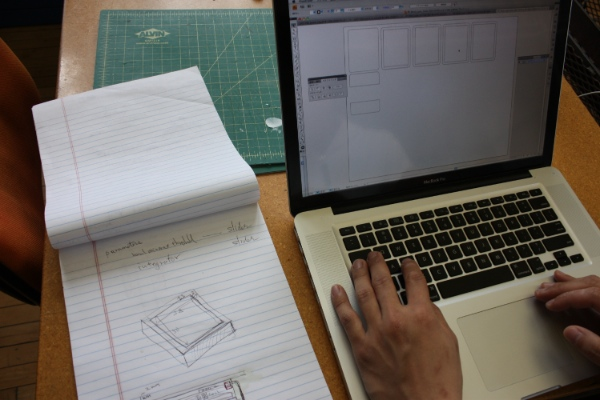
\includegraphics[width=0.9\linewidth]{img/translate-sketch-to-computer.jpg}
  \caption{A common step of designing for laser cutters: translating a
    hand-made sketch to a computer modeling tool. The sketch includes
    a perspective drawing of the desired result, and 2D diagrams of
    individual parts with key dimensions indicated.}
  \label{fig:translate}
\end{figure}

After the work practices interview, we asked participants to copy the
sketch shown in Figure~\ref{fig:interview-sketch} using a software
tool of their choice. We wanted to learn what problems people
encountered when executing the common task of translating a sketch to
a computer model.

\begin{figure}[h]
\centering \subfloat[Users were asked to replicate this sketch of a
  part.] {
  \label{fig:interview-sketch-1} 
  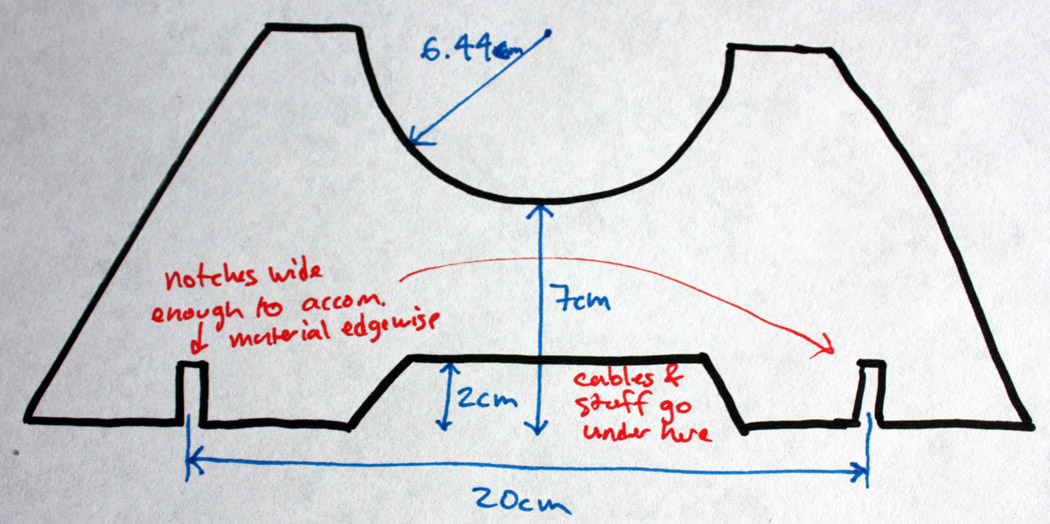
\includegraphics[width=0.9\linewidth]{img/laser-me-1.jpg}
}

\subfloat[Drawing of how the part is used in context.] {
    \label{fig:interview-sketch-2}
    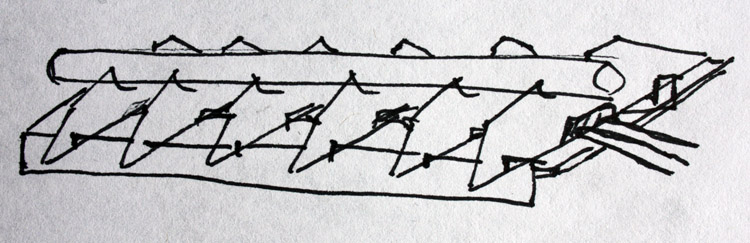
\includegraphics[width=0.9\linewidth]{img/laser-me-2.jpg}
}
\caption{We asked participants to model the part at the top using
  software.}
\label{fig:interview-sketch}
\end{figure}

Most participants chose to implement the sketch with Illustrator (5
users); one chose Rhino. Every designer's strategy involved common
activities: creating and editing boundaries, aligning or snapping
items, using guide lines or reference points, measuring distances,
specifying or changing lengths and angles, and creating finished ``cut
files'' to send to the laser cutter.  They also engaged in typical
interaction management tasks such as selecting and deselecting
on-screen elements, and view port management such as zooming and
panning.

Participants spent a good deal of time on operating overhead
(approximately 50\%). This included searching for the appropriate tool
for the next task and recovering from errors. For example, one
designer, an experienced Illustrator user, was aware of the ``Path
Finder'' tool and wanted to use it. He searched the program's menu
structure and hovered over toolbar buttons to read tool tips. Next, he
invoked various functions of the Path Finder, using the keyboard
shortcut to undo after each failed attempt, as he searched for the
correct mode within the subcommand palette. This process lasted
approximately 80 seconds.

Occasionally participants used features in unorthodox ways. For
example, to remove an unwanted segment of a polyline, one participant
(a graphic designer) created an opaque white rectangle to obscure it,
rather than erase it. (``Don't tell anyone I did this'', he said).

Similar episodes are common: a person \textit{should} know the
`correct' action, but takes an alternate approach. Although the
alternative achieves the intended effect, it might be less efficient
(more operations, longer execution time) or introduce unwanted
complexity (such as the invisible white rectangle).

To summarize, we found most common tasks and problems belong to three
main groups:

\begin{itemize}
\item \textit{Defining geometry:} Creating/editing boundaries,
  aligning items, creating and using guide lines or reference points,
  measuring distances, and specifying lengths or angles.
\item \textit{Managing the editing tool:} Selecting/deselecting
  objects, view port management, finding and entering tool modes, and
  recovering from errors.
\item \textit{Cut file:} Finalizing the cut file by creating copies of
  items when more than one is needed, and positioning stencils.
\end{itemize}

\subsection{Artifact Feature Analysis}

The formative study of work practices from the previous section helps
us understand \textit{how} people create laser cut items. To learn
more about the characteristics of those objects, we analyzed finished
items from two web-based communities of laser cutter users.

Many users are motivated by the opportunity to share their designs
with others. Ponoko and Thingiverse are two currently popular web
sites for selling or sharing items that can be made with rapid
fabrication machines. Ponoko offers thousands of user-designed items
for sale, mostly produced by laser cutting. Thingiverse is a warehouse
of digital models of 3D-printable objects and designs for laser
cutters. From these two sites we selected a total of 55 laser-cut
projects. On Ponoko we selected the most recent 50 laser cut
items. Five were later disqualified as too similar to other items. On
Thingiverse we searched for objects with the ``laser cutter'' tag. We
then examined the features of these 55
projects. Figure~\ref{fig:ponoko} summarizes the results of this
feature analysis.

\begin{figure}[h]
  \centering
  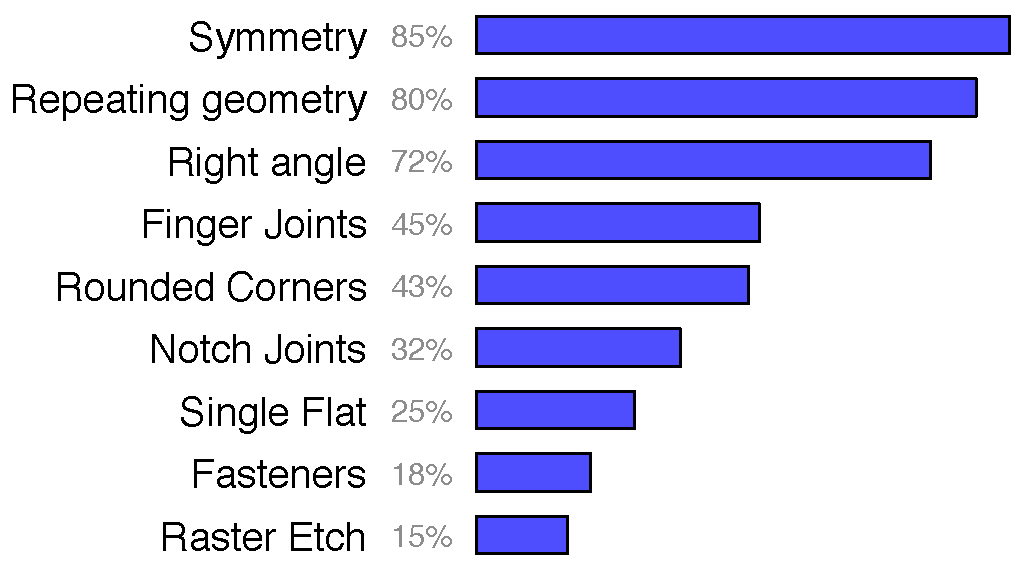
\includegraphics[width=0.9\linewidth]{img/ponoko-graph.pdf}
  \caption{Frequency of features of 55 laser-cut designs found on
    Ponoko and Thingiverse.}
  \label{fig:ponoko}
\end{figure}

We used ten properties to characterize each project, based on our own
experience designing objects for laser cutters, as well as
observations from the formative study. These properties are summarized
here and described in greater detail below:

\begin{itemize}
\item \textit{Symmetry}: Radial/linear symmetry is present.
\item \textit{Repeating geometry}: Linework is repeated several times.
\item \textit{Right Angle}: Edges meet at 90-degree angles.
\item \textit{Notch and Finger Joints}: Two parts come together using one of
  the joints illustrated in Figure~\ref{fig:joint}.
\item \textit{Rounded Corners}: Right-angle corners are slightly blunt.
\item \textit{Splines}: Curved linework (not counting rounded corners).
\item \textit{Single Flat}: The project is composed of a single, flat
  piece of material (e.g. a coaster).
\item \textit{Fasteners}: Use of glue, screws, or bolts.
\item \textit{Raster etch}: Laser cutter etched patterns (e.g. words,
  images) rather than cutting all the way through material.
\end{itemize}

\begin{figure}[h]
\centering 
\subfloat[Notch joints.] {
  \label{fig:joint-notch} 
  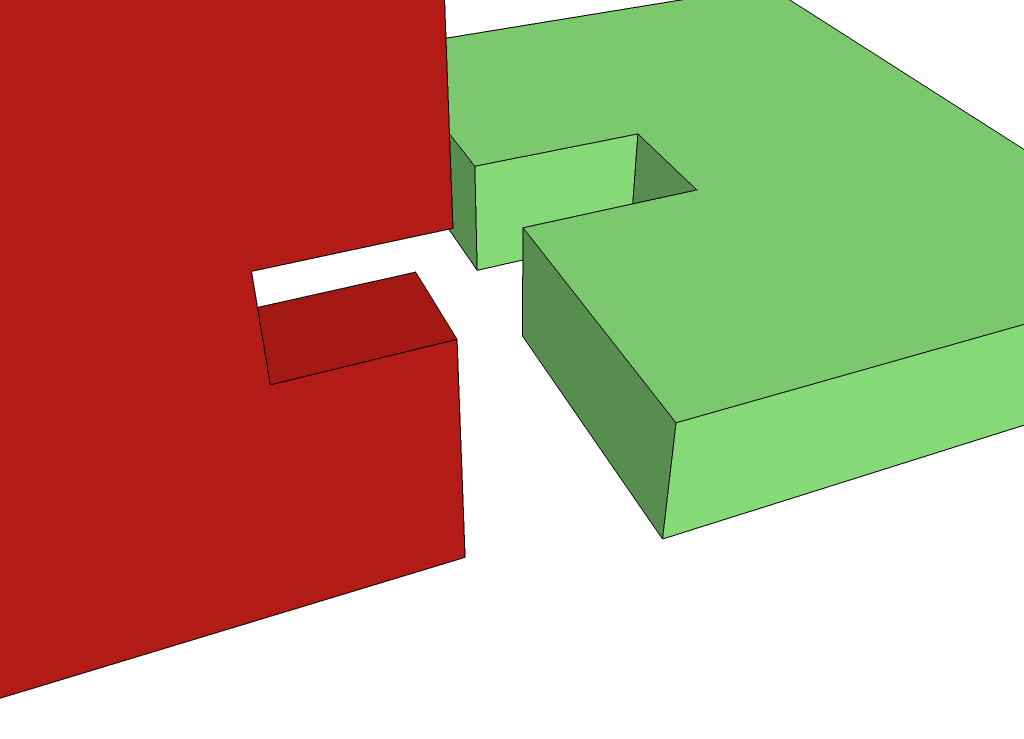
\includegraphics[width=0.4\linewidth]{img/joint-notch.png}
}
\subfloat[Finger (box) joints.] {
    \label{fig:joint-finger}
    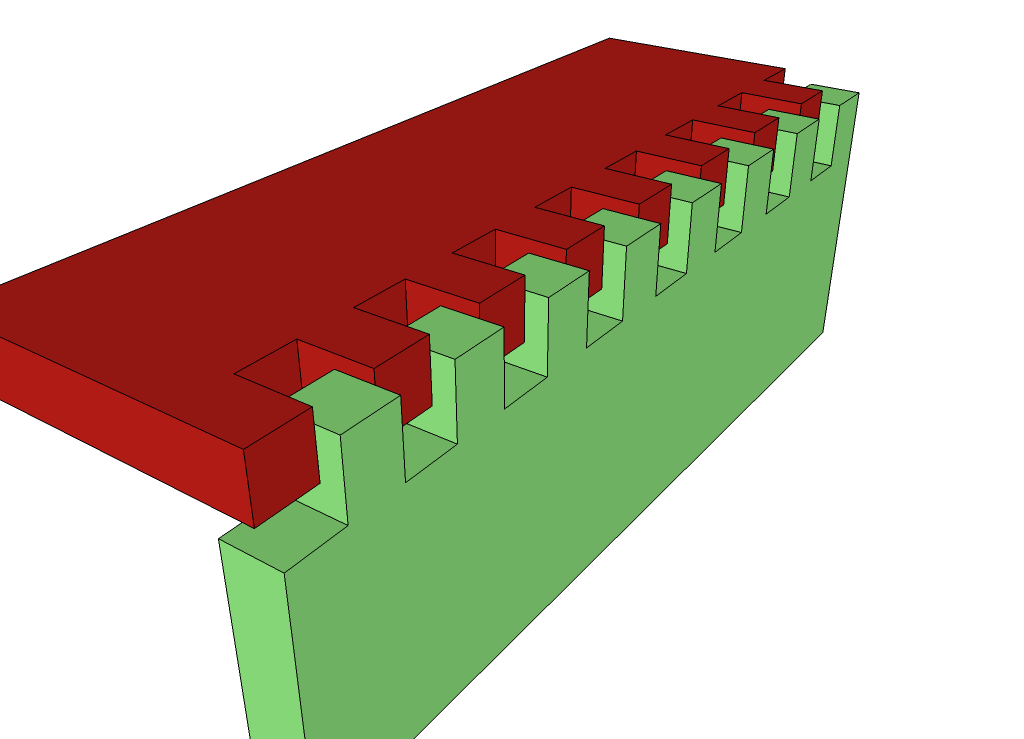
\includegraphics[width=0.4\linewidth]{img/joint-finger.png}
}
\caption{Two common methods to join parts. Notch joints are used when
  parts intersect along part midsections; finger joints (box joints)
  join parts along edges.}
\label{fig:joint}
\end{figure}

%% Single part projects were typically artistic, using expressive, curvy
%% linework. Among multi-part objects, approximately 75\% used finger or
%% notch joints (Fig.~\ref{fig:joint}). The rest used fasteners.

%% The more professional-looking models were those that used rounded
%% corners. Several designs used raster etching for artistic
%% effect. Repeating geometry was found in most models. These patterns
%% involve sequences of lines or curves with consistent length and
%% angles. Some patterns were quite ornate.

\section{SKETCH IT, MAKE IT}

Based on the designer's work practices (formative study) and the
artifacts they make (feature analysis), we developed \textit{Sketch
  It, Make It} (SIMI), a sketch-based tool for modeling laser cut
items. We aim to address problems with current modeling systems
(identified above) with a tool to specifically support designing
laser-cut items.

Design for laser cutting requires precision. The greatest distinction
between SIMI and prior sketch-based design tools is that users can
accurately specify geometry. The user may set distances and angles to
specific values. However in keeping with the spirit of sketch-based
modeling, the user is not obliged to specify details until they become
important. The systems does not \textit{require} users to attend to
detail, but enables a designer to transition from a rough imprecise
model to a specific precise model via sketch interaction.

SIMI supports precision with user-created constraints. A constraint is
a geometric relationship between two or more items. For example, two
lines can be constrained to meet at a common point, and then
constrained to meet at a right angle. These constraints are maintained
by a constraint engine as the user edits a model. Using same-length,
same-angle, and right-angle constraints users create objects with
symmetric or repeating geometry. Details on constraints and the
custom-built constraint engine are provided below.

Users draw with a stylus, and use a button with their other hand for a
few actions. We wanted to study what could be done with only a stylus
and a single button. This restrictive hardware configuration forced us
to develop techniques that might not have been found if a wider array
of hardware (e.g. multi-touch surfaces, keyboards) was an option.

The system recognizes input as either geometric linework or gestural
commands. Linework includes straight lines, elliptical arcs, splines
(open-ended or closed shapes), circles, and ellipses. Users invoke
commands to operate on linework by drawing gestures. Some gestures are
recognized and execute immediately, such as the erase (scribble)
gesture. Other gestures (like those that establish constraints) are
recognized after the user presses the button, or after a timeout.

SIMI recognizes a closed 2D path as a `stencil'. Stencils are shapes
that can be placed on the virtual laser cutter bed. Several copies of
a stencil can be added. The system generates a vector file for laser
cutting. 

\subsection{Sketch Interaction Techniques}

Guiding the development of SIMI is the principle that the designer
need never to set down the pen. Input is provided entirely with a
stylus except for a single button used by the non-dominant hand that
gives access to additional commands. The gestures used to invoke
commands or add constraints are summarized in Table~\ref{tab:gestures}
and described in detail in the following sections.

\begin{table}[h]
\centering
\begin{tabular}{ p{2.25cm} p{5.5cm} }
\textbf{Gesture} & \textbf{Remark} \\
\hline
Latching & Make segments share a common point.\\
Erase & Remove unwanted segments.\\
Same Length & Constrain line lengths to be the same.\\
Specific Length & Constrain line lengths to a value. \\
Right Angle & Constrain two lines to a $90\,^{\circ}$ angle.\\
Same Angle & Constrain two angles to be the same. \\
Flow Selection & Deform and smooth curved segments.\\
Undo and Redo & Browse and revert design history.\\
Camera Control & Zoom and pan.\\
\end{tabular}
\caption{Summary of gestures used in SIMI.}
\label{tab:gestures}
\end{table}


\begin{figure}[h]
\centering \subfloat[Automatic: latch when endcaps intersect
  (drawn in blue).] {
  \label{fig:latch-auto} 
  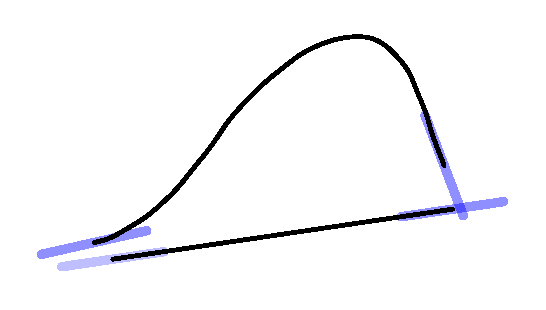
\includegraphics[width=0.43\linewidth]{img/latch-auto-endcaps.pdf}
}\hspace{5mm}
\subfloat[Manual endpoint latching.] {
  \label{fig:latch-endpoint} 
  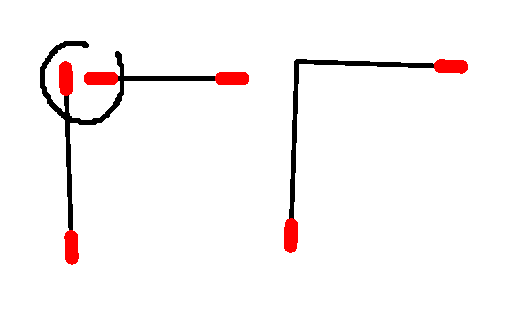
\includegraphics[width=0.43\linewidth]{img/latch-manual-endpoint.pdf}
}
\\
\subfloat[Manual continuation latching.] {
    \label{fig:latch-continuation}
    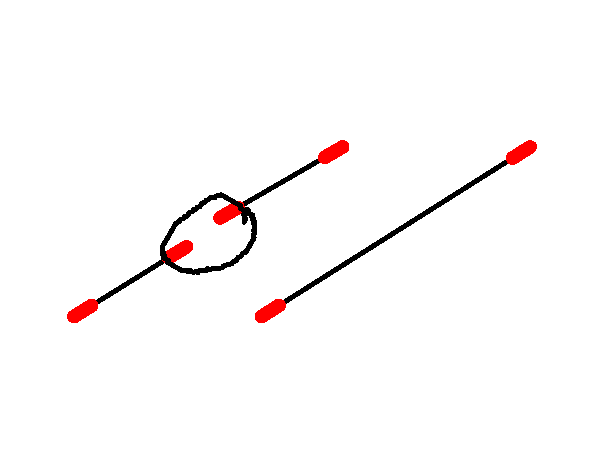
\includegraphics[width=0.43\linewidth]{img/latch-manual-continuation.pdf}
}\hspace{5mm}
\subfloat[Manual T-Junction latching.] {
    \label{fig:latch-tjunct}
    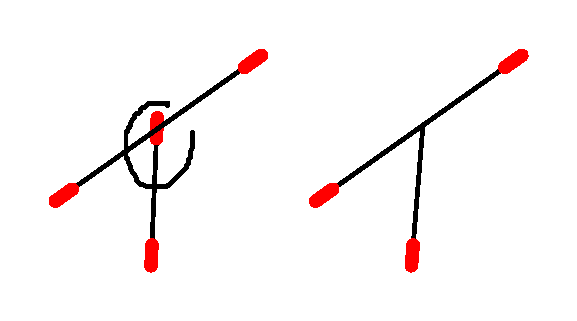
\includegraphics[width=0.43\linewidth]{img/latch-manual-tjunct.pdf}
}
\caption{Automatic and manual latching brings segments together to
  meet at a common point.}
\label{fig:latch}
\end{figure}

\subsubsection{Latching}

Users often want adjacent lines to meet at a common point. In the
formative study from the previous section, we observed Illustrator
users struggling to make lines co-terminate. Sometimes the designer
would simply extend the lines past each other to ensure the laser will
cut the corner correctly.

Latching is the process of adjusting adjacent segments (lines,
splines, arcs, \textit{etc.}) to meet at a common
point~\cite{herot-latch-corners}. SIMI provides two methods for
latching segments, illustrated in Figure~\ref{fig:latch}. One is
automatic: the system analyzes new linework for cases where the user
likely meant their segments to join together, and adjusts one or more
segments to join. Automatic latching can be problematic if it is too
zealous. Therefore our approach is intentionally conservative to avoid
frustrating users. The other latching method is manual, and is made by
drawing a small circle around the endpoints to be latched.

All linework in SIMI is meant to compose stencils, which are closed
sequences of latched segments. The designer must be able to find and
fix un-latched segments to make stencils. To reveal un-latched
segments, a red marker is drawn at lonely endpoints.

Three different spatial arrangements can be latched: endpoint
latching, continuation, and T-junctions (see
Figure~\ref{fig:latch}). Endpoint
latching~(Figure~\ref{fig:latch-endpoint}) is what the automatic
latcher does. Continuation
latching~(Figure~\ref{fig:latch-continuation}) is when the user brings
together two segments that are close to the same direction at the
joined point. Continuation latching replaces two segments with a
single larger segment. A T-junction~(Figure~\ref{fig:latch-tjunct}) is
when a segment endpoint latches to the middle of another segment,
splitting the second segment in two.

\subsubsection{Erase}

\begin{figure}[h]
  \centering
  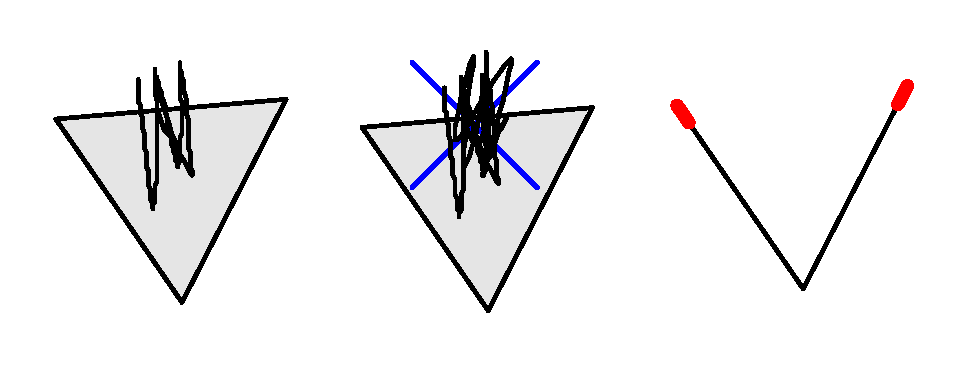
\includegraphics[width=0.9\linewidth]{img/erase-all.pdf}
  \caption{Erase gesture: before, during, and after.}
  \label{fig:erase}
\end{figure}

Users may want to remove linework for various reasons: deleting
unwanted or accidentally drawn lines, or as part of a deliberate
strategy to cut away geometry to allow new shapes to
emerge~\cite{zeleznik-lineogrammer}. Like latching, erasing is a
common task so it is invoked with a simple scribble gesture. 

Our algorithm for detecting erasure executes efficiently during the
pen stroke. When an erasure gesture is detected mid-stroke, it
provides visual feedback to give users
confidence. Figure~\ref{fig:erase} shows an erase gesture with the
visual feedback.

\subsubsection{Angle and Length Constraints}

Most laser cut stencils employ right angles, symmetry, and repeated
geometry (see Figure~\ref{fig:ponoko}). Designers can create stencils
with these properties by imposing constraints.

\begin{figure}[h]
  \centering
  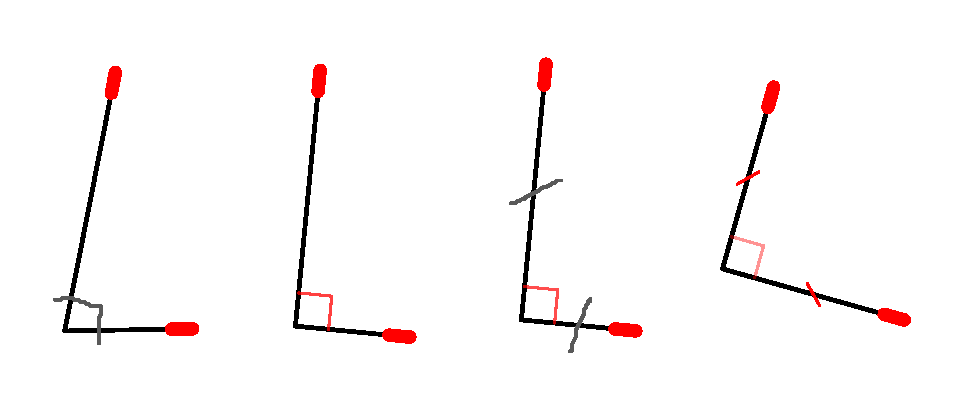
\includegraphics[width=0.9\linewidth]{img/constraints-all.pdf}
  \caption{Gestures for adding a right angle (left) and same-length.}
  \label{fig:constraints}
\end{figure}

In SIMI, designers add constraints by drawing gestures. Traditional
drafting and standard geometry diagrams indicate a right angle with a
brace symbol at the intersection of the two edges. SIMI recognizes
drawn input that looks like that brace and adds a constraint on the
associated segments (Figure~\ref{fig:constraints}).

Another drafting convention uses tick marks (hash marks) to indicate
that two lines have the same length. SIMI recognizes two or more ticks
crossing line segments as a gesture to create a \textit{same-length
  constraint}. A same-length constraint is satisfied when all segment
lengths are equal. The target length is the mean value of the
constituent lengths.

SIMI also lets designers set specific lengths, invoked by selecting a
line (by over-tracing a portion of it) and typing a number (for now we
allow keyboard input for this one case; handwriting support is future
work). If one segment in a same-length constraint is assigned a
particular length, all segments take on that length.

Angles can be constrained to be equal with the same gesture used to
make lines the same length.

\subsubsection{Flow Selection}

% Justify wrt user study and Ponoko analysis

About one-third of the models examined in our laser cut artifact
analysis involved (splines). SIMI provides Flow
Selection~\cite{johnson-flow-selection} to enable users to manipulate
create and modify splines (Figure~\ref{fig:fs}). The user `heats up'
portions of curved segments by holding the pen down near the
curve. Then, without picking up the pen, the user deforms the heated
region by dragging the pen. ``Hotter'' points along the curve move
more.

\begin{figure}[h]
\centering \subfloat[Selecting (``heating'') points along a curve near
  the stylus. The selection grows as long as the stylus is held down. ] {
  \label{fig:fs-1} 
  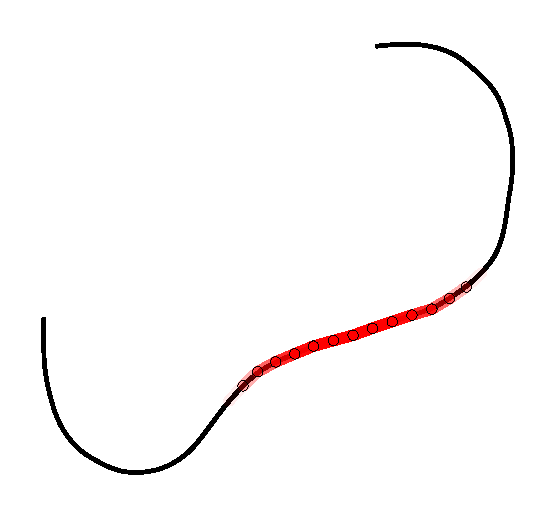
\includegraphics[width=0.4\linewidth]{img/fs-1.pdf} }
\hspace{3mm} \subfloat[Deforming the region by moving the
  stylus. ``Hotter'' points (close to the pen) are moved more than
  those farther away.] {
  \label{fig:fs-2} 
  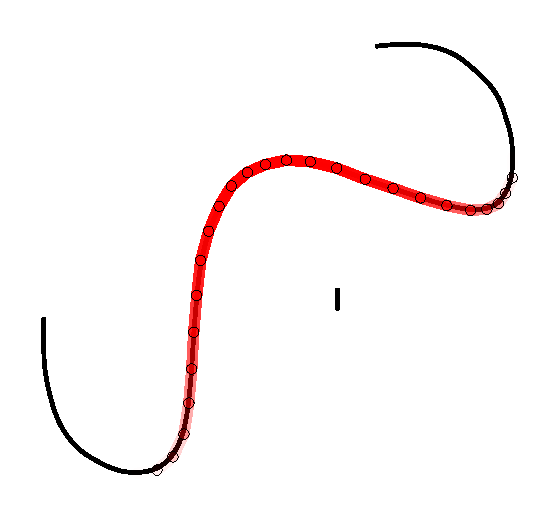
\includegraphics[width=0.4\linewidth]{img/fs-2.pdf}
}
\caption{Flow selection is used to deform curved segments. By holding
  the pen down, SIMI enters a transient mode that slowly heats the
  segment near the stylus. When the pen moves, the heated points move
  with it.}
\label{fig:fs}
\end{figure}

\subsubsection{Undo and Redo}

SIMI provides a novel means of performing Undo and Redo that lets
designers browse their entire design history. Participants in the
formative evaluation used the Undo and Redo features in two distinct
ways: to revert state following epistemic actions, or to recover from
usability problems~\cite{akers-undo}. First, Undo gives designers
confidence to modify their work to see what changes might look
like. Epistemic actions~\cite{kirsch-epistemic-action} are taken to
ask ``what if'' questions, like rotating an object 90 degrees to see
if it that orientation is better. Such actions support creative
exploration. If the designer does not like their modifications they
simply Undo to a prior state. The second class of Undo events stems
from errors: either usability problems or user error. 

Users undo by pressing the offhand button and dragging the pen to the
left. Every 40 pixels left triggers one undo action. The designer
undoes several actions by simply dragging farther to the left. Redo is
done by dragging to the right. Both undo and redo actions may be
triggered by the same stroke by changing direction, letting designers
scan the drawing history for a desired state.

\subsubsection{View Port Control}

Camera control...

\subsection{Constraint Engine}

SIMI users can establish \textit{constraints} that enforce geometric
relationships among items~\cite{borning-thinglab}. For example, the
user might draw a triangle and establish a right angle constraint. As
the user manipulates the drawing (moving vertices or changing segment
lengths), the constraint engine maintains that particular corner as a
right angle.

SIMI uses a custom-built constraint engine. It is an iterative,
numeric solver that minimizes the total error of all constraints. A
constraint's error is computed as how far each related point must move
to satisfy the constraint. However, a point may be involved in several
constraints, so it is not generally possible to simply move points to
where they satisfy one constraint because it might break one or more
other constraints. To manage contending constraints, the system
computes a change vector for each point by computing the change
required by all related constraints. Each point moves a small amount
along its change vector, and the process continues until the total
error becomes minuscule.

The solver can get trapped in a loop as points oscillate between
several values. We use simulated annealing~\cite{metropolis-annealing}
to avoid this case: points move randomly, and move more when there is
more entropy. Gradually the system reduces the level of randomness and
the points settle to a satisfactory configuration.

\subsection{Stencils}

SIMI's final product is a ``cut file'': a vector drawing for a laser
cutter. This cut file typically contains a number of stencils---closed
2D shapes that define the laser's path. Stencils may have complex
boundary geometry with non-intersecting edges. Stencils can also have
any number of holes in them, for joints, fasteners, or other purposes.

To identify stencils, SIMI forms a graph with segments as edges and
their endpoints as nodes. It then runs a depth-first search. Cycles
from a given point is a candidate stencil. Stencils are visually
represented by shading the interior.

\section{SYSTEM EVALUATION}

We evaluated Sketch It, Make It in two ways. First, we conducted a
workshop with 60 undergraduate architecture students to gather
feedback about how useful and usable it was, and to solicit other
comments. Our objective was to validate if (and how well) SIMI's
sketch-based interaction could be used to make precisely-defined
designs for fabrication.

Second, we compare experienced SIMI user's strategy for making an
object with that of an experienced Illustrator user. This was done to
compare how these starkly different tools require designers to work.

\begin{figure}[t]
\centering \subfloat[Questions on feature ease of use.] {
  \label{fig:survey-feature-ease} 
  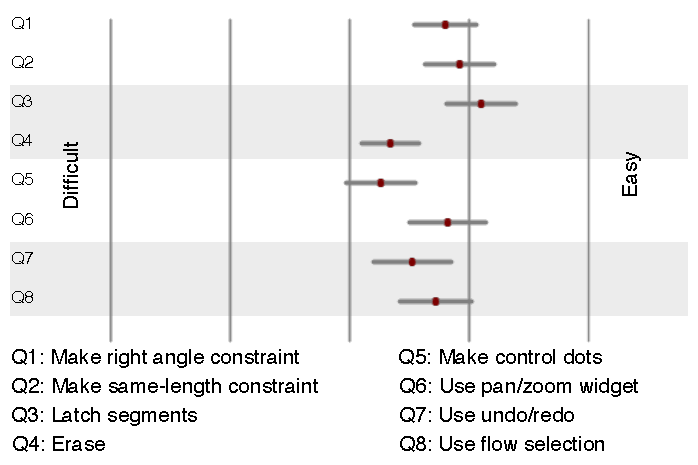
\includegraphics[width=0.8\linewidth]{img/feature-ease-of-use.pdf}
}
\\
\subfloat[Questions on how well liked (or disliked) features were.] {
    \label{fig:survey-feature-attitude}
    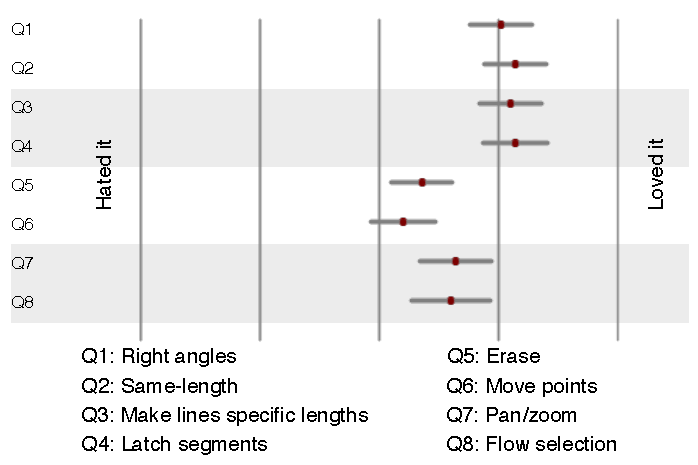
\includegraphics[width=0.8\linewidth]{img/feature-attitude.pdf}
}
\\
\subfloat[Questions on the system as a whole.] {
    \label{fig:survey-program-attitude}
    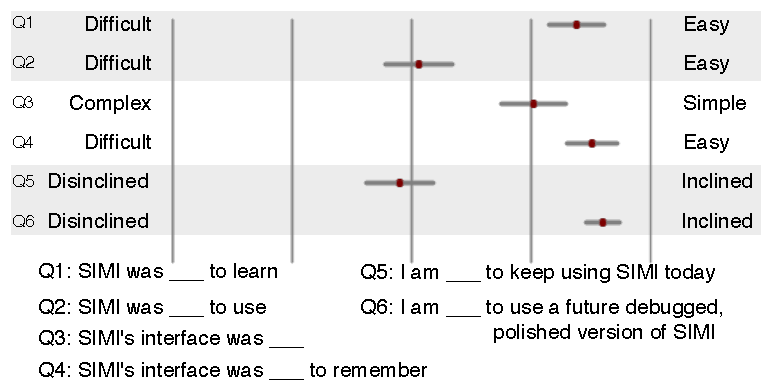
\includegraphics[width=0.8\linewidth]{img/program-attitude.pdf}
}
\caption{Survey results from the workshop with undergraduate
  architecture students. 40 students responded to the questionnaire.}

\label{fig:survey}
\end{figure}

\subsection{Student Workshop}

We held a workshop with 60 undergraduate architecture students to
gather qualitative feedback about how easy or difficult SIMI is to
learn and use. The primary author ran the workshop, held as two
30-minute sessions over two days in a room equipped with iMacs and
Wacom Intuos tablets. These tablets do not display output, so users
eyes are not focused on the same physical location as the pen
tip---leading to hand-eye coordination challenges. Display tablets
like the Cintiq (Figure~\ref{fig:cintiq}) do not have this problem.

Initially, students complained that the tablet hardware was difficult
to use, but they acclimated to it after about ten minutes. Then they
quickly learned to make linework and make constraints. At first they
had trouble erasing and using control points, but soon learned to use
these features.

%% The students had access to a video demonstrating how various
%% techniques were performed, as well as a paper ``cheat sheet'', but did
%% not use them. Instead, the students would ask somebody (e.g. the
%% author, or the student next to them) who knew how to do it. Personal
%% help was superior because assistance could be tailored to their
%% particular needs.

We expected students to have difficulty using SIMI because the
hardware (tablets) and interaction paradigm (sketch-based modeling)
were both new to them. However, by the second day, most questions and
comments regarded missing features, not about how to use the system.

After the workshop, students were offered an extra credit assignment
to complete a short survey. This generated 40 responses, summarized in
Figure~\ref{fig:survey}. The survey had three sets of questions, all
on a 5-point scale. The first set asked how easy (or hard) each
interaction method was to use. The second set of questions measured
the student's attitude about the techniques. This line of questioning
was borrowed from~\cite{bae-everybody}.

Only the Erase and Control Dot gestures seemed to give participants
trouble. These are the only gestures that incorporate timing. Erasing
must be done with a quick, vigorous shake of the pen. Control dots
must be made quickly, or SIMI will interpret the input as the
beginning of a flow selection.

The last set of questions polled students about their perception of
the program as a whole: e.g. how easy it was to learn, to use, and
remember. Although the students reported the system was easy to learn,
their responses indicate they found it difficult to use. This might be
explained by both the limited time available (each user had only one
hour), and the novelty of the hardware.

Finally, we asked (1) how much people would like to continue using the
system as it is currently, and (2) how likely they would be to try it
again when it was debugged and nicely tuned. The responses are in
stark contrast: most did not want to continue using SIMI as it is
today, owing to bugs and lack of features. Despite this, the response
to the second question was very positive (mean: 4.5, std. dev: 0.55).

The enthusiasm about the interaction paradigm of sketching was evident
in comments left by some of the respondents. For example:

\begin{itemize}
\item ``This is the start of a great program, and once it is polished it
  will be extremely useful.''
\item ``The program seems like it could be really cool to use in the
  future. I really enjoyed using a tablet and stylus. It made
  designing fun.''
\end{itemize}

Not all commentary was positive. Aside from bug-related comments, most
negative comments concerned missing features (for example, students
wanted a constraint to make lines parallel).

\subsection{Task-Tool Analysis}

A second method to evaluate our system is to compare the actions
required to make an object with SIMI compared with an existing
tool. This analysis is meant to illustrate how SIMI is different from
(and similar to) existing tools. 

We asked an expert Adobe Illustrator user to verbally describe the
sequence of discrete actions necessary to model the parts of the table
shown in Figure~\ref{fig:table}. This designer has years of experience
as an architect and has made dozens, if not hundreds, of laser-cut
items using Illustrator.

The first three actions were: (1) press the M key to enter rectangle
drawing mode, (2) type rectangle dimensions, and (3) place the
rectangle on the drawing canvas. The first action is a persistent mode
change, while the second two specify values. A similar transcript was
recorded for SIMI (the primary author provided the protocol). 

We identified discrete actions from the verbal protocol, and coded
each using five categories:

\textit{Persistent mode change}: Change the tool input state so
subsequent input is interpreted in context of that tool (e.g. line
drawing mode). User must enter another persistent mode to exit the
first.

\textit{Specify value}: Specify a dimension or location.

\textit{Specify target}: Indicate (select) an element for a subsequent
operation.

\textit{Transformation}: Apply an operation that changes existing
model elements (e.g. move or erase something)

\textit{Transient mode change}: Temporarily change the tool mode so
input is interpreted differently. This kind of mode change is part of
a phrase, and will revert to another mode when the phrase is complete.

\begin{figure}[h]
  \centering
  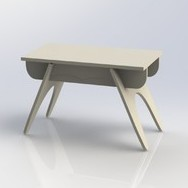
\includegraphics[width=0.4\linewidth]{img/table.jpg}
  \caption{A laser-cut table for sale on Ponoko. We asked expert
    designers how they would replicate this object using either
    Illustrator or SIMI.}
  \label{fig:table}
\end{figure}

\begin{table}[h]
\centering
\begin{tabular}{ l c c }
\textbf{Action type} & \textbf{Illustrator} & \textbf{SIMI} \\
\hline
Persistent mode change & 12 & 0 \\
Specify value & 17 & 7 \\
Specify target & 7 & 4 \\
Transformation & 6 & 27 \\
Transient mode change & 2 & 0 \\
\hline
& \textbf{44} & \textbf{38} \\
\end{tabular}
\caption{Frequency of action types in the design protocol of expert
  Adobe Illustrator and SIMI users. }
\label{tab:expert}
\end{table}

The action frequency (listed in Table~\ref{tab:expert}) shows how the
two tools are used to create the same output. Roughly the same number
of actions was taken in both cases (Illustrator:~44, SIMI:~38).

To make an object using Illustrator, an expert issues a series of
\textit{Select, Specify} actions: either enter a persistent tool
(e.g. line mode) mode or select a modeling element (e.g. a line on the
screen), then specify a value or position by typing a number or moving
the mouse.

In contrast, most discrete actions with SIMI involve transforming
geometry that is already on the screen, for example, constraining two
existing lines to meet at a common point or form a right angle. A
single sketched gesture fluidly performs both \textit{Select} and
\textit{Specify} operations that require two distinct actions in
Illustrator. For example, right angle gesture necessarily indicates
the line segments to be constrained.

\section{IMPLEMENTATION}

SIMI is programmed in approximately 20,000 lines of Java code. It uses
the Java binding for OpenGL (JOGL) for graphics and NIST's JAMA
package for linear algebra. When packaged as a self-contained
executable, the Mac OS X application is 8.2 megabytes.

\section{FUTURE WORK}

\begin{itemize}
\item handwriting recognition for lengths
\item support variables and expressions for lengths
\item shape replacement
\item additional constraints: parallel, specific-angle
\item 'hints': recognition of new ink is guided by selection
\item move/rotate/scale objects (based on undergrad feedback)
\end{itemize}

\section{CONCLUSION}

Conclusion...

\section{ACKNOWLEDGMENTS}

% TODO: fill this in later. Leave left blank for blind review.

Acknowledgments...

\bibliography{simi}

\end{document}
